\begin{center}

  \begin{tabular}{rp{16cm}lp{20cm}}%{rl}

  % after \\: \hline or \cline{col1-col2} \cline{col3-col4} ...

  论文地址:& \href{https://arxiv.org/pdf/2106.00750.pdf}{https://arxiv.org/pdf/2106.00750.pdf} \\
  来源:& ICLR, 2021 \\
  作者:& Sana Tonekaboni, Danny Eytan, Anna Goldenberg \\

  源码:& \href{https://github.com/sanatonek/TNC_representation_learning}{TNC} \\

%  slides:& \href{http://yunshengb.com/wp-content/uploads/2017/03/nips_2018_r2l_workshop_talk.pdf}{{\footnotesize Convolutional Set Matching for Graph Similarity}}\\

  关键词:& \textbf{time series, unsupervised representation learning} \\

  写于:& \date{2021-06-16}

  \end{tabular}

\end{center}

该论文\cite{tonekaboni2020unsupervised}针对的是(非平稳)时间序列数据的无监督表征问题,论文的Motivation来自Heathcare领域,患者的状态会在不同的临床状态之间转移。文中采用了对比学习的思想。

\paragraph{问题定义}
给定一个时间序列样本$X \in R^{D \times T}$,其中$T$该样本所跨越的时间长度,$D$表示样本在每一个时间步的特征维度。$X_{\left[t-\frac{\delta}{2}, t+\frac{\delta}{2}\right]}$表示$X$上的长度为$\delta$的时间窗口,因为该窗口以$t$为中心,我们表示为$W_t$。论文要解决的问题就是通过无监督学习得到$W_t$的表征。

\paragraph{TNC思路}
\begin{figure}[h]
	\centering
	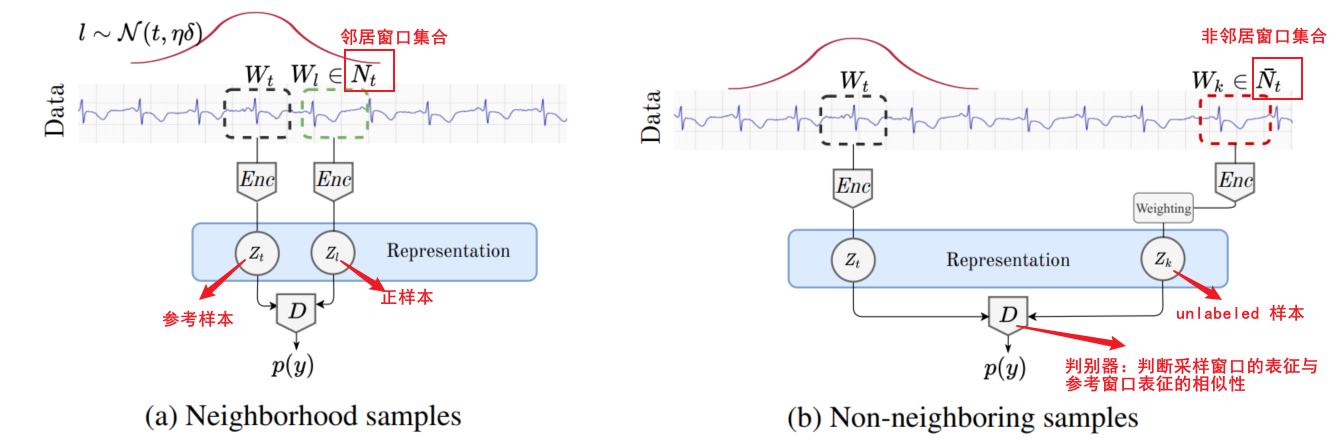
\includegraphics[width=.9\textwidth]{pics/tnc.png}
	\caption{TNC Architecture}
	\label{fig:tnc}
\end{figure}
TNC框架如Fig.\ref{fig:tnc}所示。在问题定义中已经看到,论文是要学习一个时间窗口的表征,加上论文中使用了对比学习,因此很容易想到:对于一个$W_t$,需要采样正样本$W_l$与负样本$W_k$。既然如此,怎么采样就成了一个关键问题。

文中定义了\textbf{$W_t$的Temporal Neighborhood($N_t$)},以及Non Temporal Neighborhood($\bar{N_t}$)。显而易见,$W_l \in N_t, \: W_k \in \bar{N_t}$。既然如此,那么怎么定义Temporal Neighborhood呢?

说明白了,$N_t, \bar{N_t}$都是窗口的集合,那么只要给定窗口长度以及窗口中心就确定了一个窗口,通常窗口长度都是固定的,那么只需要确定窗口中心即可。论文中对$N_t$中的窗口中心$t^*$定义为:$t^{*} \sim \mathcal{N}(t, \eta \cdot \delta)$,其中$\eta$表示邻居的范围(\textbf{有点不解}),$\delta$表示窗口长度。作为时间序列的信号,通常有一个假设:信号局部是平稳的,即是光滑的。因此$N_t$中的窗口与$W_t$相似。$\eta$对于每个$t$都是不同的,$\eta$要尽量反映出信号保持静止(大致静止)的时间跨度,因此论文中使用了 Augmented Dickey-Fuller (ADF) 统计检验来为每个$W_t$计算$\eta$。

$\bar{N_t}$的采样,则是从与$t$有一定距离(从代码中可以看出这个距离是和$\eta$有关的)的范围内采样得到的。论文中并没有直接将$\bar{N_t}$中的样本当作负样本。原因是sample bias:从数据分布中随机采样的负样本有可能与参考样本是相似的。论文中将$ W_k \in \bar{N_t}$视作unlabeld 样本。从实践的角度来看:用一个参数$w$表示unlabeled 样本属于正样本的概率,因此一个unlabeled样本表示$w$个正样本与$1-w$个负样本的结合,在计算损失的时候,unlabeled 样本会分别作为正负样本与参考样本计算损失,再分别乘以$w, 1-w$作为这个unlabeled样本的损失。

$$
\mathcal{L}=-\mathbb{E}_{W_{t} \sim X}\left[\mathbb{E}_{W_{l} \sim N_{t}}[\log \underbrace{\mathcal{D}\left(Z_{t}, Z_{l}\right)}_{\mathcal{D}\left(\operatorname{Enc}\left(W_{t}\right), \operatorname{Enc}\left(W_{l}\right)\right)}]+\mathbb{E}_{W_{k} \sim \bar{N}_{t}}[\left(1-w_{t}\right) \times \log \underbrace{\left(1-\mathcal{D}\left(Z_{t}, Z_{k}\right)\right)}_{\mathcal{D}\left(\operatorname{Enc}\left(W_{t}\right), \operatorname{Enc}\left(W_{k}\right)\right)}+w_{t} \times \log \mathcal{D}\left(Z_{t}, Z_{k}\right)]\right]
$$

\textbf{流程}:获取一个参考样本$W_t$,在获取一个正样本$W_l$以及一个unlabeled样本$W_k$,分别传入一个编码器(通常是序列模型,可以是RNN,因为每个样本就是一个时间序列样本)中,分别得到表征$Z_t, Z_l, Z_k$。用一个判别器(其实就是一个分类器)分别计算$(Z_t, Z_l), \:(Z_t, Z_l)$一个分数(该样本对相似的度量),再计算对比损失,特别要注意$(Z_t, Z_l)$的损失哦!

\paragraph{总结}

\begin{itemize}

	\item 文中对unlabeled的想法很有趣
	\item 文中的实验通过聚类以及trajactory来发现序列随时间的变化,这也是我之前考虑过的一个问题
	\item 不知道用在图数据集上怎么样,挖掘图数据的变化,可以是graph-level的或者是node-level的

\end{itemize}

